%%%%%%%%%%%%%%%%%%%%%%%%%%%%%%%%%%%%%%%%%%%%%%%%%%%%%%%%%%%%%%%%%%%%%%
%%  Copyright by Wenliang Du                                        %%
%%  This work is licensed under the Creative Commons                %%
%%  Attribution-NonCommercial-ShareAlike 4.0 International License. %%
%%  To view a copy of this license, visit                           %%
%%  http://creativecommons.org/licenses/by-nc-sa/4.0/.              %%
%%%%%%%%%%%%%%%%%%%%%%%%%%%%%%%%%%%%%%%%%%%%%%%%%%%%%%%%%%%%%%%%%%%%%%

\newcommand{\commonfolder}{../../common-files}

\documentclass[11pt]{article}

\usepackage[most]{tcolorbox}
\usepackage{times}
\usepackage{epsf}
\usepackage{epsfig}
\usepackage{amsmath, alltt, amssymb, xspace}
\usepackage{wrapfig}
\usepackage{fancyhdr}
\usepackage{url}
\usepackage{verbatim}
\usepackage{fancyvrb}
\usepackage{adjustbox}
\usepackage{listings}
\usepackage{color}
\usepackage{subfigure}
\usepackage{cite}
\usepackage{sidecap}
\usepackage{pifont}
\usepackage{mdframed}
\usepackage{textcomp}
\usepackage{enumitem}


% Horizontal alignment
\topmargin      -0.50in  % distance to headers
\oddsidemargin  0.0in
\evensidemargin 0.0in
\textwidth      6.5in
\textheight     8.9in 

\newcommand{\todo}[1]{
\vspace{0.1in}
\fbox{\parbox{6in}{TODO: #1}}
\vspace{0.1in}
}


\newcommand{\unix}{{\tt Unix}\xspace}
\newcommand{\linux}{{\tt Linux}\xspace}
\newcommand{\minix}{{\tt Minix}\xspace}
\newcommand{\ubuntu}{{\tt Ubuntu}\xspace}
\newcommand{\setuid}{{\tt Set-UID}\xspace}
\newcommand{\openssl} {\texttt{openssl}}


\pagestyle{fancy}
\lhead{\bfseries SEED Labs}
\chead{}
\rhead{\small \thepage}
\lfoot{}
\cfoot{}
\rfoot{}


\definecolor{dkgreen}{rgb}{0,0.6,0}
\definecolor{gray}{rgb}{0.5,0.5,0.5}
\definecolor{mauve}{rgb}{0.58,0,0.82}
\definecolor{lightgray}{gray}{0.90}


\lstset{%
  frame=none,
  language=,
  backgroundcolor=\color{lightgray},
  aboveskip=3mm,
  belowskip=3mm,
  showstringspaces=false,
%  columns=flexible,
  basicstyle={\small\ttfamily},
  numbers=none,
  numberstyle=\tiny\color{gray},
  keywordstyle=\color{blue},
  commentstyle=\color{dkgreen},
  stringstyle=\color{mauve},
  breaklines=true,
  breakatwhitespace=true,
  tabsize=3,
  columns=fullflexible,
  keepspaces=true,
  escapeinside={(*@}{@*)}
}

\newcommand{\newnote}[1]{
\vspace{0.1in}
\noindent
\fbox{\parbox{1.0\textwidth}{\textbf{Note:} #1}}
%\vspace{0.1in}
}


%% Submission
\newcommand{\seedsubmission}{You need to submit a detailed lab report, with screenshots,
to describe what you have done and what you have observed.
You also need to provide explanation
to the observations that are interesting or surprising.
Please also list the important code snippets followed by
explanation. Simply attaching code without any explanation will not
receive credits.}

%% Book
\newcommand{\seedbook}{\textit{Computer \& Internet Security: A Hands-on Approach}, 2nd
Edition, by Wenliang Du. See details at \url{https://www.handsonsecurity.net}.}

%% Videos
\newcommand{\seedisvideo}{\textit{Internet Security: A Hands-on Approach},
by Wenliang Du. See details at \url{https://www.handsonsecurity.net/video.html}.}

\newcommand{\seedcsvideo}{\textit{Computer Security: A Hands-on Approach},
by Wenliang Du. See details at \url{https://www.handsonsecurity.net/video.html}.}

%% Lab Environment
\newcommand{\seedenvironment}{This lab has been tested on our pre-built
Ubuntu 16.04 VM, which can be downloaded from the SEED website. }

\newcommand{\seedenvironmentA}{This lab has been tested on our pre-built
Ubuntu 16.04 VM, which can be downloaded from the SEED website. }

\newcommand{\seedenvironmentB}{This lab has been tested on our pre-built
Ubuntu 20.04 VM, which can be downloaded from the SEED website. }

\newcommand{\seedenvironmentAB}{This lab has been tested on our pre-built
Ubuntu 16.04 and 20.04 VMs, which can be downloaded from the SEED website. }

\newcommand{\nodependency}{Since we use containers to set up the lab environment, 
this lab does not depend too much on our SEED VM. You can do this lab
using other VMs or physical machines. }







\newcommand{\seedlabcopyright}[1]{
\vspace{0.1in}
\fbox{\parbox{6in}{\small Copyright \copyright\ {#1}\ \ by Wenliang Du.\\
      This work is licensed under a Creative Commons
      Attribution-NonCommercial-ShareAlike 4.0 International License.
      If you remix, transform, or build upon the material, 
      this copyright notice must be left intact, or reproduced in a way that is reasonable to
      the medium in which the work is being re-published.}}
\vspace{0.1in}
}




% Copyright 2017 Sergei Tikhomirov, MIT License
% https://github.com/s-tikhomirov/solidity-latex-highlighting/

%\usepackage{listings, xcolor}

\lstdefinelanguage{Solidity}{
	keywords=[1]{anonymous, assembly, assert, balance, break, call, callcode, case, catch, class, constant, continue, constructor, contract, debugger, default, delegatecall, delete, do, else, emit, event, experimental, export, external, false, finally, for, function, gas, if, implements, import, in, indexed, instanceof, interface, internal, is, length, library, log0, log1, log2, log3, log4, memory, modifier, new, payable, pragma, private, protected, public, pure, push, require, return, returns, revert, selfdestruct, send, solidity, storage, struct, suicide, super, switch, then, this, throw, transfer, true, try, typeof, using, value, view, while, with, addmod, ecrecover, keccak256, mulmod, ripemd160, sha256, sha3}, % generic keywords including crypto operations
	keywordstyle=[1]\color{blue}\bfseries,
	keywords=[2]{address, bool, byte, bytes, bytes1, bytes2, bytes3, bytes4, bytes5, bytes6, bytes7, bytes8, bytes9, bytes10, bytes11, bytes12, bytes13, bytes14, bytes15, bytes16, bytes17, bytes18, bytes19, bytes20, bytes21, bytes22, bytes23, bytes24, bytes25, bytes26, bytes27, bytes28, bytes29, bytes30, bytes31, bytes32, enum, int, int8, int16, int24, int32, int40, int48, int56, int64, int72, int80, int88, int96, int104, int112, int120, int128, int136, int144, int152, int160, int168, int176, int184, int192, int200, int208, int216, int224, int232, int240, int248, int256, mapping, string, uint, uint8, uint16, uint24, uint32, uint40, uint48, uint56, uint64, uint72, uint80, uint88, uint96, uint104, uint112, uint120, uint128, uint136, uint144, uint152, uint160, uint168, uint176, uint184, uint192, uint200, uint208, uint216, uint224, uint232, uint240, uint248, uint256, var, void, ether, finney, szabo, wei, days, hours, minutes, seconds, weeks, years},	% types; money and time units
	keywordstyle=[2]\color{teal}\bfseries,
	keywords=[3]{block, blockhash, coinbase, difficulty, gaslimit, number, timestamp, msg, data, gas, sender, sig, value, now, tx, gasprice, origin},	% environment variables
	keywordstyle=[3]\color{violet}\bfseries,
	identifierstyle=\color{black},
	sensitive=false,
	comment=[l]{//},
	morecomment=[s]{/*}{*/},
	commentstyle=\color{gray}\ttfamily,
	stringstyle=\color{red}\ttfamily,
	morestring=[b]',
	morestring=[b]"
}



\hypersetup{%
    pdfborder = {0 0 0}
}


\lhead{\bfseries SEED Labs -- Smart Contract Lab}

\begin{document}

\begin{center}
{\LARGE Smart Contract Lab}
\end{center}

\seedlabcopyright{2023}

\newcommand{\contractfolder}{{\path{Labsetup/contract}}\xspace}

% *******************************************
% SECTION
% ******************************************* 
\section{Overview}

A smart contract is a program that runs on a
blockchain. Its code, which is immutable and 
stored at a particular address of the blockchain, 
gets executed automatically
when a predetermined condition is met. 
Its data (state) is also stored on the blockchain. 
The objective of this lab is to help students understand how 
this type of program works and how to write 
simple smart contract code. 
Students will conduct experiments on the 
SEED blockchain emulator using the 
provided smart contract code.
The following topics are covered in this lab: 

\begin{itemize}[noitemsep]
\item Smart contract development 
\item Remix IDE
\item Deploy and interact with smart contract
\item Send fund to and from smart contract
\end{itemize}
 

\paragraph{Lab environment.} The activities in this document 
have been tested on our pre-built
Ubuntu 20.04 VM, which can be downloaded from the SEED website.  


% *******************************************
% SECTION
% *******************************************
\section{Lab Setup: Starting the Blockchain Emulator}

This lab will be performed inside the SEED Internet Emulator (simply
called the emulator in this document). If this is the first time you
use the emulator, it is important that you read this section.
We recommend instructors to provide a lab session to
help students get familiar with the emulator.




\paragraph{Download the emulator files.}
Please download the \texttt{Labsetup.zip} file from the web page, and
unzip it. You will get the emulator files. 
The emulator consists of a number of container files, which are stored 
in the \path{Labsetup/emulator_*} folders. The \texttt{emulator\_NN}
folders are for AMD64 machines, while the \texttt{emulator\_arm\_NN}
are for the Apple silicon machines. The number 
\texttt{NN} represents the number of nodes on the blockchain network:
students can choose the smaller one if the RAM given for their virtual 
machine is less than 4GB. 


To run the emulator, we 
only need these container files. These files are generated using
the Python code stored in the \path{Labsetup/emulator_code} folder. 
Unless you want to modify the emulator files, you do not 
need to run the code in this folder (you need to 
install the SEED Emulator library from the GitHub to run the code). 
Instructors who would like to customize the emulator can modify the Python
code and generate their own emulator files.

For the sake of simplicity, the blockchain running inside the emulator
uses the Proof-of-Authority (PoA) consensus protocol, instead of the
Proof-of-Stake protocol used in the MAINET. 
The activities conducted in this lab are not dependent on 
any specific consensus protocol.


\paragraph{Start the emulator.}
Go to the \texttt{emulator} folder, and run the following docker commands
to build and start the containers. The commands listed below are aliases 
created on the SEED VM.
If you are not using the SEED VM, you can use
the original commands. 

\begin{lstlisting}
$ dcbuild       # Alias for: docker-compose build
$ dcup          # Alias for: docker-compose up
\end{lstlisting}

We recommend that you run the emulator inside
the provided SEED Ubuntu 20.04 VM, but doing it in a generic Ubuntu 20.04 
operating system
should not have any problem, as long as the docker software is installed.
For newer operating system version, the \texttt{docker-compose} command 
has already been phased out; it is integrated into the \texttt{docker}
command, and you can run it using \texttt{"docker compose"},
instead of \texttt{docker-compose}.  
Readers can find the docker manual from
\href{https://github.com/seed-labs/seed-labs/blob/master/manuals/docker/SEEDManual-Container.md}
{\underline{this link}}.
If this is the first time you set up a SEED lab environment
using containers, it is very important that you read 
the user manual. 




All the containers will be running in the background. To run
commands on a container, we often need to get a shell on
that container. We first need to use the \texttt{"docker ps"}  
command to find out the ID of the container, and then
use \texttt{"docker exec"} to start a shell on that 
container. We have created aliases for them in
the \texttt{.bashrc} file.

\begin{lstlisting}
$ dockps        // Alias for: docker ps --format "{{.ID}}  {{.Names}}" 
$ docksh <id>   // Alias for: docker exec -it <id> /bin/bash

// The following example shows how to get a shell inside hostC
$ dockps
b1004832e275  hostA-10.9.0.5
0af4ea7a3e2e  hostB-10.9.0.6
9652715c8e0a  hostC-10.9.0.7

$ docksh 96
root@9652715c8e0a:/#  

// Note: If a docker command requires a container ID, you do not need to 
//       type the entire ID string. Typing the first few characters will 
//       be sufficient, as long as they are unique among all the containers. 
\end{lstlisting}





If you encounter problems when setting up the lab environment, 
please read the ``Common Problems'' section of the manual
for potential solutions.


\paragraph{Stop the emulator.} 
To stop the emulator, we just need to stop all the containers. 
We can go to the terminal where we run the 
\texttt{"docker-compose up"} command, type \texttt{Ctrl-C}.
That will stop all the containers, but without removing them, i.e., all the data 
in the containers are still preserved, and they can be resumed by 
running \texttt{"docker-compose up"} again. 
If we want to remove them, we can run the \texttt{"docker-compose down"}
command. Another way to do this is to go to a different terminal (but still in the
same \texttt{emulator} folder) and directly run this command.  
That will stop and removing all the containers.

\begin{lstlisting}
$ dcdown        # Alias for: docker-compose down
\end{lstlisting}






\paragraph{EtherView.}

We have implemented a simple web application called \texttt{EtherView} to
display the activities on the Blockchain. To access the application,
point your browser (within the VM) to \url{http://localhost:5000/}.
From the \texttt{Blocks} page, you can see the newly created blocks and 
recent transactions. If nobody is sending transactions, the 
blocks are mostly empty, i.e., containing no transactions. Once we 
start sending transactions, we should be able to see them. 
Users can click on the blocks and transactions to see their details.







% *******************************************
% SECTION
% *******************************************
\section{Task 1: Using Remix for Smart Contract Development} 

There are several development environments for smart contracts, including
Hardhat, Remix, and Truffle. In this lab, we will use 
Remix IDE (Integrated Development Environment), which can be
used to write, compile, and debug the Solidity code. 
It supports testing, debugging and deploying smart contracts. 


% -------------------------------------------
% SUBSECTION
% -------------------------------------------
\subsection{Task 1.a: Connecting Remix to the SEED Emulator} 

Remix IDE has an online version and a desktop version. 
We will use the online IDE, so there is no need to install anything. 
Simply go to this URL \url{https://remix.ethereum.org/}, and you 
will get the Remix IDE. Remix provides excellent instructions on 
how to use the IDE at this URL \url{https://remix-ide.readthedocs.io/}. 


Remix can connect to blockchain via several mechanisms,
such as Remix VM, injected provider (MetaMask), and external HTTP
providers. The Remix VM is sandbox blockchain in the browser;
it simulates the behavior of a blockchain, so 
it is not a real blockchain.
We will connect Remix to our SEED blockchain emulator, which
is a real blockchain (a private blockchain). This can be done using an injected 
provider (such as MetaMask) or an external HTTP provider. 


We will use MetaMask in this task. We first connect MetaMask
to the SEED blockchain emulator, and then tell Remix to use
MetaMask whenever it needs to interact with the blockchain. 
MetaMask not only serves as our bridge to the blockchain, it is 
also a wallet: whenever we need to send a transaction,
we have to do that from an account; we use MetaMask
to manage our accounts. 

In the Blockchain exploration lab, we have already installed
MetaMask extension to our browser. If you have not done that
lab before, you can follow the instruction in 
this URL to set it up:\url{https://github.com/seed-labs/seed-labs/blob/master/manuals/emulator/metamask.md}. To restore the 
accounts, please use the following mnemonic phrase:


\begin{lstlisting}
gentle always fun glass foster produce north tail security list example gain
\end{lstlisting}
 

After setting up MetaMask, go to the Remix IDE, 
in the \texttt{"Deploy \& Run Transactions} menu,
set the \texttt{Environment} to \texttt{"Injected Provider - MetaMask"}.  
If everything is set up correctly, in the \texttt{Account} drop-down menu,
you should be able to see several accounts with balance. 


% -------------------------------------------
% SUBSECTION
% -------------------------------------------
\subsection{1.b: Write, Compile, and Deploy Smart Contract} 

In this task, we will use Remix to deploy a simple smart contract
called \texttt{Hello.sol}. The code can be found in 
the \contractfolder folder.


\begin{itemize}
\item \textit{Writing code}: Go to the \texttt{Workspaces} menu 
in Remix, and you will see several folders.
Inside the \texttt{contract} folder, create a new file called 
\texttt{Hello.sol}. Copy and paste the content 
of the provided \texttt{Hello.sol} file to this new file.  


\item \textit{Compiling code}: Go to the \texttt{"Solidity compiler"} menu,
and compile the \texttt{Hello.sol} program.  

\item \textit{Deploying contract}:  Go to the \texttt{"Deploy \& run 
transactions"} menu and click the \texttt{Deploy} button.  
MetaMask will come up and ask you to confirm. If you do not see 
MetaMask, check your \texttt{Environment} setting to make sure 
that MetaMask is selected. If the deployment is successful,
you should be able to see the confirmation from MetaMask.
Go to EtherView and show that your deployment transaction has 
been added to a block. 

\end{itemize}


% -------------------------------------------
% SUBSECTION
% -------------------------------------------
\subsection{1.c: Under the hood}

In this task, we will see what really happens when we deploy a contract.
Deploying a contract is done through a transaction, which is 
different from fund-transfer transaction. 
Please deploy a contract, and then use EtherView to get the transaction
details. Compare this transaction with a fund-transfer transaction,
and describe the main differences between these two types of 
transactions. In the contract-deployment transaction, you 
will see some content in the data field contain. What is 
this content? Please provide evidence to support your conclusion. 


\paragraph{Note:} In this task, you may need to get the 
bytecode of a compiled contract. This can be obtained from
Remix. In the \texttt{"Solidity Compiler"} menu, you should be 
able to see the \texttt{ABI} and \texttt{Bytecode} buttons. 
You can also go to the \contractfolder folder,
compile the code using the provided \texttt{Makefile}.   
You can get the bytecode. 



% *******************************************
% SECTION
% *******************************************
\section{Task 2: Invoke Contract Functions} 

In this task, we will see how to interact with a smart contract.
We will use the \texttt{Hello} contract deployed from the previous 
task. Go to the \texttt{"Deployed Contracts"} region,  
and we should be able to see the contracts that were
just deployed, including their addresses, balances,
and the functions. 


% -------------------------------------------
% SUBSECTION
% -------------------------------------------
\subsection{Task 2.a: Invoke a function via local call} 

If a function is defined as a \texttt{"public view"} type, 
it does not modify the state of the contract, and is thus 
invoked through a local call, instead of via a transaction. 
There is no cost for this type of interaction. Remix creates a button 
for this type of function, as well as for the \texttt{public} 
variable (for each \texttt{public} variable, a default getter function of 
the \texttt{"public view"} type is created). 
We can interact with the contract using these buttons. 
Please invoke all the \texttt{"public view"} functions of the contract,
and report your observation. 


% -------------------------------------------
% SUBSECTION
% -------------------------------------------
\subsection{Task 2.b: Invoke a function via transaction} 

If a function modifies the sate of the contract, it has to 
be invoked via a transaction. Remix uses a different 
color for the buttons corresponding to these functions. 
Please invoke the \texttt{increaseCounter()} function,
and report your observation. Please uses EtherView
to show the transactions generated by this invocation. 

Add a new function called \texttt{decreaseCounter(unit)} 
function to the smart contract. Compile and Deploy it.
Interact with this new function and show your results. 





% -------------------------------------------
% SUBSECTION
% -------------------------------------------
\subsection{Task 2.c: Under the hood} 
\label{subsec:under_the_hood}


What has actually happened when we send a transaction to 
invoke a function? Please take a look at the \texttt{to} and  
the \texttt{data} fields of such a transaction, and 
explain their meanings. 
To invoke a function, we need to provide the function name
and arguments. This information is encoded in the 
the \texttt{data} field.
Please invoke the \texttt{increaseCounter()} function, 
get the transaction details using EtherView, and then
verify whether the \texttt{data} field is indeed encoded 
based on the following: 

\begin{itemize}[noitemsep]
\item Function selector: The first 4 bytes of the hash of the 
      function’s prototype
\item Arguments: encoded according to the types defined in ABI (32 bytes each)
\end{itemize}
 
The following Python script help you calculate the hash of a 
function's prototype. 

\begin{lstlisting}
from web3 import Web3

hash = Web3.sha3(text="<function signature>")
print(hash.hex())
\end{lstlisting}


After understanding what really happens, let us invoke a function
directly through the data field, instead of using the buttons provided
by Remix (those buttons actually construct the content for the data field). 
In Remix, at the bottom of the \texttt{"Deployed contract} region,  
you can see a region called \texttt{"Low level interactions"}.
Whatever we put in the \texttt{CALLDATA} field will be 
put in the \texttt{data} field of the transaction.  
Please use this method to invoke the \texttt{increaseCounter()}
function, and verify that the invocation is successful. 


% -------------------------------------------
% SUBSECTION
% -------------------------------------------
\subsection{Task 2.d: Emit events} 


Smart contracts can emit events to communicate that something has happened on the
blockchain. Applications can listen to these events and take actions 
when they happen. In \texttt{Hello.sol}, we have declared an
event called \texttt{MyMessage}. Then in the \texttt{sendMessage()}
function, we use \texttt{emit} to generate a message. 

\begin{lstlisting}
event MyMessage(address indexed _from, uint256 _value);

function sendMessage() public returns (uint256) {
   emit MyMessage(msg.sender, counter);
   return counter;
}
\end{lstlisting}


The generated messages are placed inside the log field of 
a transaction receipt. By monitoring this field, an application
can be notified. Remix does display the log field. Please 
take a look at the field, and confirm that its content is 
what you have expected. 
 

%\paragraph{TODO:} 
%Write a python program to monitor a particular 
%type of events. Query the node every 5 seconds.




% *******************************************
% SECTION
% *******************************************
\section{Task 3: Send Fund to Contract} 

In this task, we will send fund to a contract. 
We will use a different contract for this task. 
The contract program is called \texttt{EtherFaucet.sol}, and 
it can be found in the \contractfolder folder.  
Please copy and paste the Solidity source code to Remix, 
compile it, and then deploy it to the SEED blockchain. 

When we send fund to a smart contract, some of the contract's 
function (must be the \texttt{payable} type) 
will be invoked. Depending on the situation, different 
functions will be invoked. Figure~\ref{fig:payable_function}
depicts the conditions for invoking each function. 
In this task, we will conduct experiments
for each of the situations. 

\begin{figure}[htb]
\begin{center}
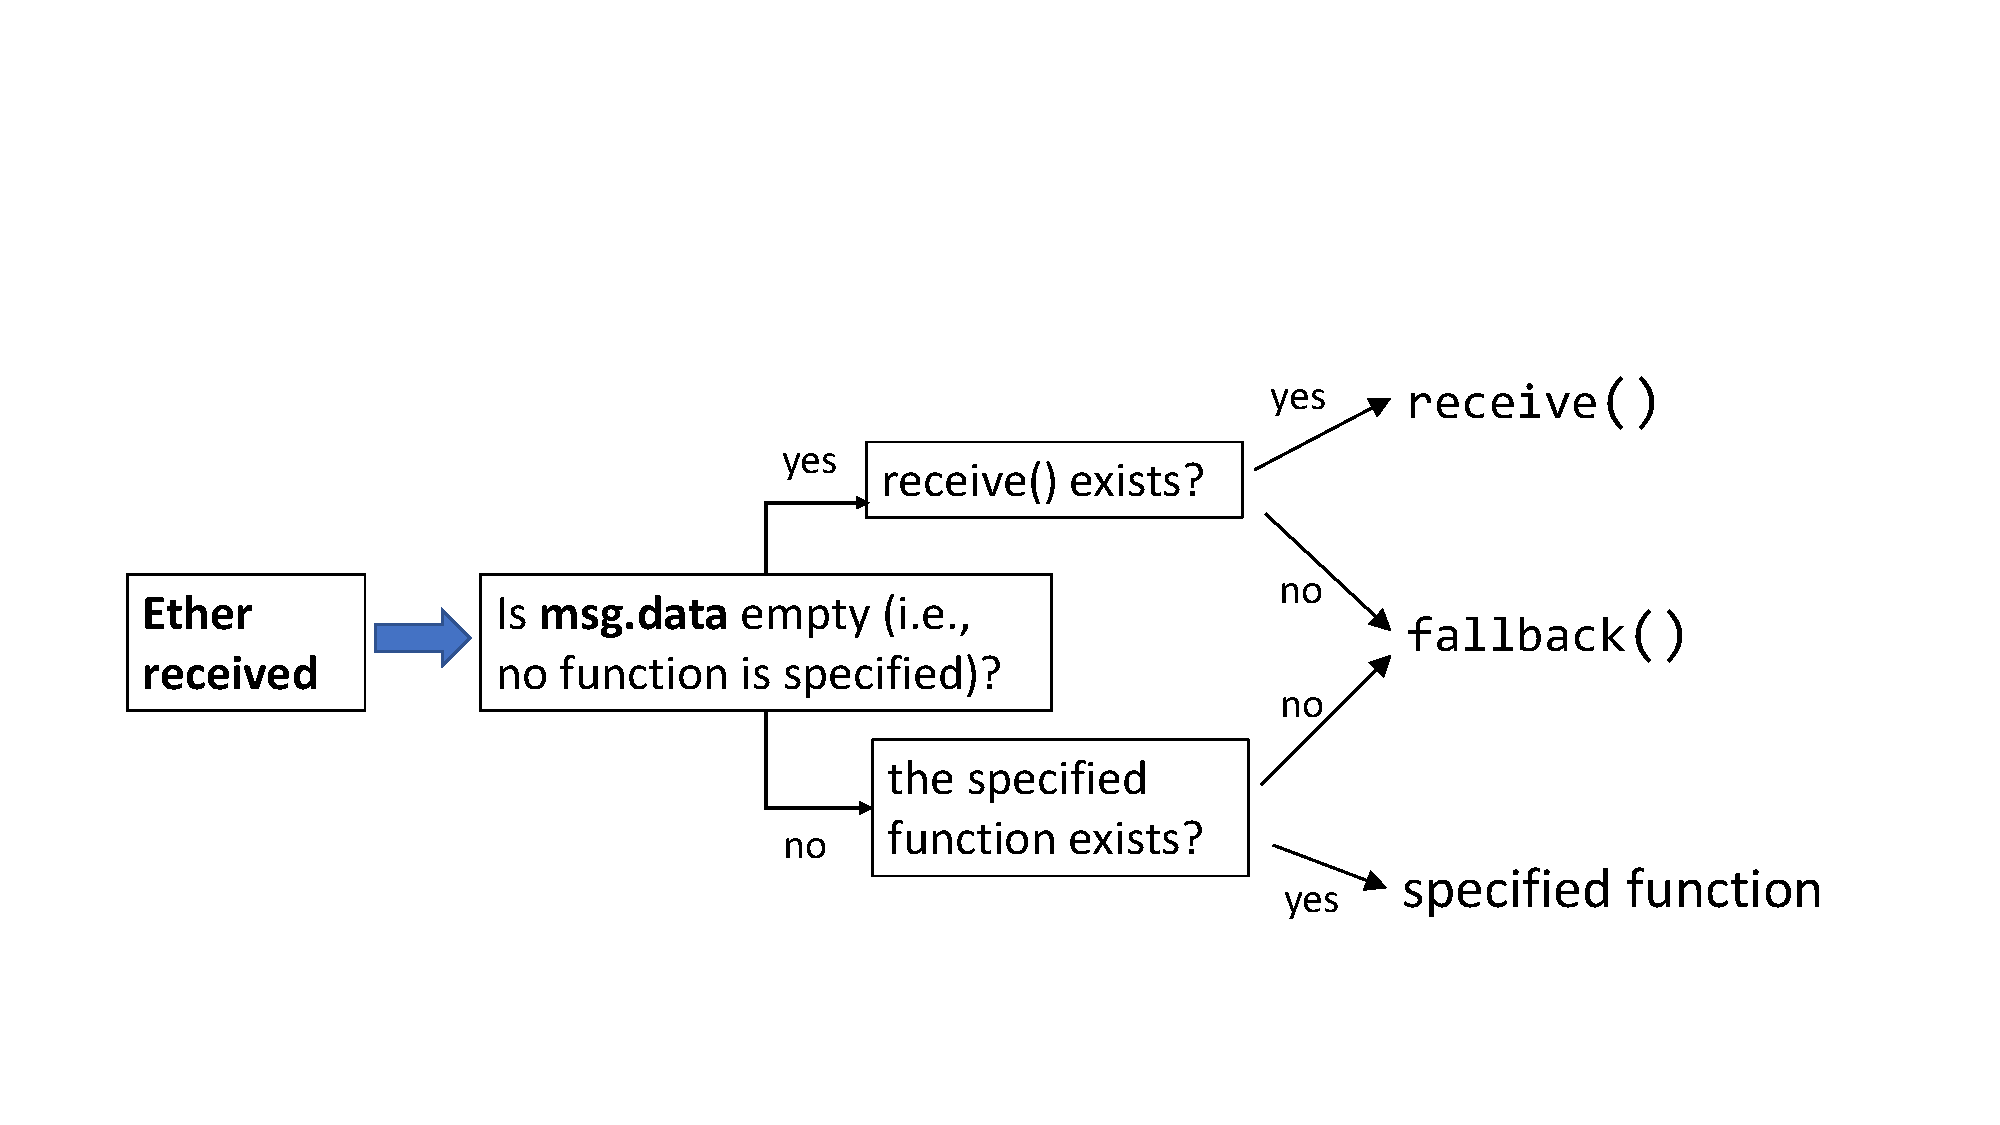
\includegraphics[width=0.65\textwidth]{Figs/send_fund.pdf}
\end{center}
\caption{Which payable function is invoked when fund is sent to a contract}
\label{fig:payable_function}
\end{figure}
 

% -------------------------------------------
% SUBSECTION
% -------------------------------------------
\subsection{Task 3.a: Send fund directly to a contract address} 

One can directly directly send fund to a contract using the contract's 
address. This is done through a regular transaction. 
In this case, we are not specifying any function to invoke 
in our transaction. However, when a contract receives the fund,
one of its function will be invoked. 


Please use MetaMask to send some fund to the \texttt{EtherFaucet}
contract using its address. Once the transaction has been confirmed,
check the balance of the smart contract on Remix. 
The \texttt{amount} variable should contain the same value as the 
balance (in different unit). Conduct the following experiments:


\begin{itemize}[noitemsep]
\item Check the \texttt{count} variable of the contract to verify 
that the function invoked is consistent with what is 
described in Figure~\ref{fig:payable_function}. 

\item Try to remove the \texttt{receive()} function from the 
contract, and see what warnings Remix will be giving. 
\end{itemize}
 


% -------------------------------------------
% SUBSECTION
% -------------------------------------------
\subsection{Task 3.b: Send fund to a payable function} 

We can send fund to a contract while invoking
a payable function. We will do this from Remix and
invoke the \texttt{donateEther()} function
to send some Ethers to the contract. How much is sent 
to the contract is specified in the \texttt{value}
field of the transaction. You need to put some amount 
in this field (which is displayed above the \texttt{Deploy}
button). The function invoked can get the fund amount
using \texttt{msg.value}. 
After the invocation, please verify that the values 
of the balance, the \texttt{amount} variable and 
the \texttt{donationCount} variable are what 
is expected. 

\begin{lstlisting}
function donateEther() external (*@\textbf{payable}@*) {
    amount += (*@\textbf{msg.value}@*);
    donationCount += 1;
}
\end{lstlisting}
 

% -------------------------------------------
% SUBSECTION
% -------------------------------------------
\subsection{Task 3.c: Send fund to a non-payable function} 

Function that can receive funds must be \texttt{payable}.
Please try to remove the \texttt{payable} keyword 
from the \texttt{donateEther()} function and see what warnings Remix 
will be giving. We also provided a function called 
\texttt{donateEtherWrong()}, which is not \texttt{payable}.
Please send some fund to the contract via invoking 
this function. You may receive some warnings, but 
do ignore them and send out the transaction. What will 
happen? Will the fund transfer succeed? Will
the sender lose money if it does not succeed? 

\begin{lstlisting}
function donateEtherWrong() external {
    donationCount += 1;
}
\end{lstlisting}
 

% -------------------------------------------
% SUBSECTION
% -------------------------------------------
\subsection{Task 3.d: Send fund to a non-existing function}

In this task, we will send fund to a contract while invoking 
a function. However, we intentionally make a mistake 
by invoking a function that does not exist in the contract. 
We will see what will actually happen. 

To invoke a non-existing function, we will directly 
set the \texttt{data} field of our transaction. 
As what we did in \ref{subsec:under_the_hood}, 
we can use the \texttt{"Low level interactions"} of 
Remix to directly set the \texttt{data} field. 
Let us invoke a function called \texttt{foo()}, which
does not exist in the contract. We will send some fund
to the contract while invoking this function. Please 
show what happens. Will the fund sending successful? 
What function will be invoked? etc. 
 


% *******************************************
% SECTION
% *******************************************
\section{Task 4: Send Fund from Contract}

In the previous task, we see how to send fund to a contract. In this 
task, we will see how to send fund from a contract to a recipient. 
In Solidity, there are three different methods for sending ether 
from a contract, including
\texttt{send}, \texttt{transfer}, and \texttt{call}.    
All three methods are translated into the CALL opcode by the 
Solidity compiler, so they share the same internal process, but
they have differences. 
Regarding which one is recommended to use, the 
existing documentation on the Internet has been quite confusing 
because of the constant changes of the Ethereum blockchain.

%One difference is the propagation of exceptions, the transfer() method 
%automatically revert of all state changes if there is an error. 
%The send() and call() however return false in case of an error,
%leaving the decision to revert state changes or not to the 
%program logic. 

The major difference among these three methods is the 
gas limit forwarded to the recipient. 
When a transaction is sent, a gas limit is set by the 
original sender. When this transaction invokes a contract A, which
triggers the contract to send ether to a recipient, 
if the recipient is also a contract (say B), some of B's 
code will be executed. B needs some gas to run, and how much gas
it gets depends on how much is forwarded by the sender contract A. 

The \texttt{send} and \texttt{transfer} methods set a limit 
of fixed 2300 gas forwarded to the recipient, 
With this limited gas, B cannot do much. The main reason for placing such a limit 
is to prevent the reentrancy attack (which is covered by another SEED lab). 
The \texttt{call} by default does not have such a limit, i.e., it 
forwards all the gas set by the original sender. 
We can also set a limit when using \texttt{call} method. 

Due to the changes of the blockchain, the gas costs of the code 
might change, and the 2300 gas limit might not be sufficient in the future. 
This may cause some smart contract applications to break. 
Therefore, suggestions have been
made to not to use the \texttt{send} and \texttt{transfer} 
method. Instead, use the \texttt{call} method. Although the 
\texttt{call} method is subject to the reentrancy attack,
there are many ways to prevent such an attack. 
Actually, after the Istanbul hardfork,
the \texttt{send} and \texttt{transfer} methods have been deprecated.

%This is where many things can go wrong. 
%This lab does not cover all the secure practice, as it focuses only on 
%the mechanisms. We will develop future labs to cover the security
%aspect. The Reentrancy attack lab is one of such labs. 


%Regarding forwarding gas: The gas that is not used by the recipient is returned to the sender
%contract, and the gas that it does not use is then refunded to the original sender. This way,
%previous senders can continue doing more operations.



\paragraph{Task: Send fund to an external owned account.} 
We have implemented the send-fund functionality 
in our \texttt{EtherFaucet} contract using all these three methods. 
Please use Remix to invoke each of these methods, and see 
whether you can receive ether from the contract. 
It should be noted that the \texttt{\_amount} argument 
uses the wei as its unit, so if we want to get one ether, 
we should use \texttt{1e18} as the amount. 

\begin{lstlisting}
function getEtherViaCall(uint256 _amount) external payable {
    address payable to = payable(msg.sender);
    amount -= _amount;
    (bool success, ) = (*@\textbf{to.call\{value: \_amount\}("")}@*);
    require(success, "Failure: Ether not sent");
}

function getEtherViaSend(uint256 _amount) external payable {
    address payable to = payable(msg.sender);
    amount -= _amount;
    bool success = (*@\textbf{to.send(\_amount)}@*);
    require(success, "Failure: Ether not sent");
}

function getEtherViaTransfer(uint256 _amount) external payable {
    address payable to = payable(msg.sender);
    amount -= _amount;
    (*@\textbf{to.transfer(\_amount)}@*);
}
\end{lstlisting}
 
It should be noted that in this sample code, everybody can get
any amount of ether from this contract, so this is definitely 
not secure. In a real smart contract, access control should be 
placed to ensure only authorized accounts can receive fund 
from this contract. Also, for the sake of simplicity, 
we did not put any protection against the reentrancy attack 
in the code. 
We have a separate SEED lab on the reentrancy attack. 


% *******************************************
% SECTION
% *******************************************
\section{Task 5: Invoke Another Contract} 

Inside a contract, we can invoke the functions of another contract. 
In this task, we will see how such an invocation works. 
We have provided a smart contract called \texttt{Caller.sol}, 
which can be found from the \contractfolder folder. 
We will use it to invoke the functions in the \texttt{Hello.sol} 
contract, which was deployed in Task 1. 

The code snippet is listed below. It needs to include an 
\texttt{interface} derived from the \texttt{Hello} contract.
This way, we can create a contract object, and then use
the APIs in the interface to interact with the 
\texttt{Hello} contract. We have provided two 
invocation examples. The only difference is that 
one only does the invocation, and the other 
also sends fund to the \texttt{Hello} contract
during the invocation. 


\begin{lstlisting}
function invokeHello(address addr, uint _val) public returns (uint) {
   Hello c = Hello(addr);
   uint256 v =  c.increaseCounter(_val);

   emit ReturnValue(msg.sender, v);
   return v;
}

function invokeHello2(address addr, uint _val) public onlyOwner 
                                               returns (uint) 
{
   Hello c = Hello(addr);
   uint256 v =  c.increaseCounter2{value: 1 ether}(_val);
                                             (*@\pointupleft{send fund}@*) 
   emit ReturnValue(msg.sender, v);
   return v;
}

interface Hello {
    function sayHello() external pure returns (string memory);
    function getResult(uint a, uint b) external view returns (uint);
    function increaseCounter(uint k) external returns (uint);
    function increaseCounter2(uint k) external payable returns (uint); 
    function getCounter() external view returns (uint);
    function sendMessage() external returns (uint256);
}
\end{lstlisting}
 

\paragraph{Task.} Please deploy the \texttt{Caller} contract,
and invoke its \texttt{invokeHello()} and \texttt{invokeHello2()} 
functions. Please describe your 
observation and explain what you see. 




\begin{comment} % No need to include this
% -------------------------------------------
% SUBSECTION
% -------------------------------------------
\subsection{Task 5.b: Send fund to another contract} 

Using the \texttt{call()} method, we can also send  
Send to the \texttt{Hello.sol} contract deployed in Task 1. 
Invoke \texttt{sendEtherToAddress()} function of the 
\texttt{EtherFaucet.sol} contract, while setting the 
\texttt{Hello.sol} contract's address as the \texttt{\_to} 
argument. 

\begin{lstlisting}
function sendEtherToAddress(uint256 _amount, address payable _to) external payable {
    amount -= _amount;
    (bool success, ) = _to.call{value: _amount}("");
    require(success, "Failure: Ether not sent");
}
\end{lstlisting}
\end{comment} 



% *******************************************
% SECTION
% ******************************************* 
\section{Submission}

\seedsubmission


\end{document}



